% ---------------------------------------------------------------------------
% Appendix: CALSPEC spectrophotometric validation of the Custom Colors
% photometry pipeline.
%
% Drop this file into the paper with % ---------------------------------------------------------------------------
% Appendix: CALSPEC spectrophotometric validation of the Custom Colors
% photometry pipeline.
%
% Drop this file into the paper with % ---------------------------------------------------------------------------
% Appendix: CALSPEC spectrophotometric validation of the Custom Colors
% photometry pipeline.
%
% Drop this file into the paper with % ---------------------------------------------------------------------------
% Appendix: CALSPEC spectrophotometric validation of the Custom Colors
% photometry pipeline.
%
% Drop this file into the paper with \input{appendix_calspec.tex} (and move
% the figure files into the paper's figures directory, or adjust the path in
% \includegraphics below).
% ---------------------------------------------------------------------------

\section{CALSPEC Spectrophotometric Validation}
\label{app:calspec}

The demonstrations in Section~\ref{sec:demonstrations} test the combined
photometric pipeline (atmosphere grid, interpolation, filter convolution, zero
point) against real-star photometry.  The residuals they probe are therefore a
sum of contributions from each of those steps.  To isolate the pieces that
\textsc{Custom Colors} actually implements -- the filter convolution and the
zero-point calibration -- this appendix compares synthetic magnitudes computed
directly from the CALSPEC spectrophotometric standards \citep{Bohlin2014,
Bohlin2019, Bohlin2020} against their published magnitudes in Gaia DR3, 2MASS,
and Johnson systems.  Because the input spectra are the empirical HST STIS
and NICMOS/WFC3 flux distributions rather than atmosphere-grid interpolants,
the comparison is independent of the atmosphere coverage, the Hermite
interpolation scheme, and any evolutionary model.

\subsection{Method}

We selected 17 CALSPEC primary standards spanning $T_{\rm eff} \approx$ 2700~K
(the M7V dwarf VB~8) through $\approx 60{,}000$~K (the DA white dwarf
G191--B2B), and including the Vega reference itself, three primary DA white
dwarfs (G191--B2B, GD~71, GD~153), four solar analogs (P330-E, P177-D,
18~Sco, 16~Cyg~B), hot DO/sdO standards (Feige~34, Feige~110, HZ~43), the
exoplanet host HD~209458, two early-type stars (109~Vir, 10~Lac), and two
cool/ultracool benchmarks (VB~8, 2MASS~J00361617+1821104).  For each star we
downloaded the current (2024) CALSPEC FITS release from the
STScI\footnote{\url{https://ssb.stsci.edu/cdbs/current_calspec/}} archive.

For each (star, filter) pair we evaluate the synthetic Vega-system magnitude
\begin{equation}
    m_X = -2.5 \log_{10}\!\left(\frac{F_{X,\mathrm{star}}}{F_{X,\mathrm{Vega}}}\right).
\end{equation}
Critically, both $F_{X,\mathrm{star}}$ and $F_{X,\mathrm{Vega}}$ are computed
by calling the \emph{same} \textsc{Custom Colors} Fortran kernels that run
inside \textsc{mesa} during a stellar evolution, exposed through the
\texttt{sed\_model.cc\_api} interface
(Section~\ref{sec:sed_model}).  No Python reimplementation of the band
integration or the zero-point calibration is used: the Python driver loads the
spectra and the filter curves, applies the detector-type conversion required
by \texttt{colors\_utils.f90:load\_filter} when the header reports
\verb+DetectorType=energy+, and then invokes
\texttt{cc\_api.synthetic\_magnitude} and \texttt{cc\_api.vega\_zero\_point}
on the resulting arrays.  This ensures that the validation targets the
production photometry pipeline rather than a surrogate.

The Vega reference is the shipped CALSPEC Vega spectrum \citep{Bohlin2020}
resampled onto each filter grid.  The filter curves themselves are those
distributed with \textsc{Custom Colors} in
\texttt{data/colors\_data/filters/} and (for 2MASS) with the companion
\texttt{SED\_Tools} package.  Published magnitudes used for
the comparison are: Gaia DR3 \texttt{Gmag}, \texttt{BPmag}, and \texttt{RPmag}
\citep{GaiaDR3}; the 2MASS All-Sky Point Source Catalog
\citep{2mass_cutri}; and Johnson $V$ and $B-V$ from the CALSPEC literature
tables \citep{Bohlin2014, Bohlin2019}.  Residuals are reported as $\Delta m
\equiv m_{\rm synth} - m_{\rm published}$ in mmag.

Because several of the CALSPEC standards are either bright enough to saturate
the 2MASS catalog (Vega, 16~Cyg~B, 10~Lac) or faint and intrinsically red
beyond the regime where the Gaia DR3 processing is well calibrated (VB~8, 2MASS
J00361617+1821104), we also report a \emph{reliable} subset defined by (i) a
CALSPEC spectrum that spans at least 99 per cent of the integrated filter
support in every band tested, and (ii) a published uncertainty $\sigma_m \le
50$~mmag in the band under comparison.  The reliable set comprises 10
standards: BD+17~4708, G191--B2B, GD~71, GD~153, HD~209458, HZ~43, Feige~34,
Feige~110, P330-E, and P177-D.

\subsection{Results}

Table~\ref{tab:calspec_residuals} reports the residual statistics for the
reliable set, and Figure~\ref{fig:calspec_residuals} shows the per-band
residuals as a function of $T_{\rm eff}$ with the published catalog
uncertainties as error bars.

\input{table_calspec_residuals.tex}

\begin{figure*}[t]
    \centering
    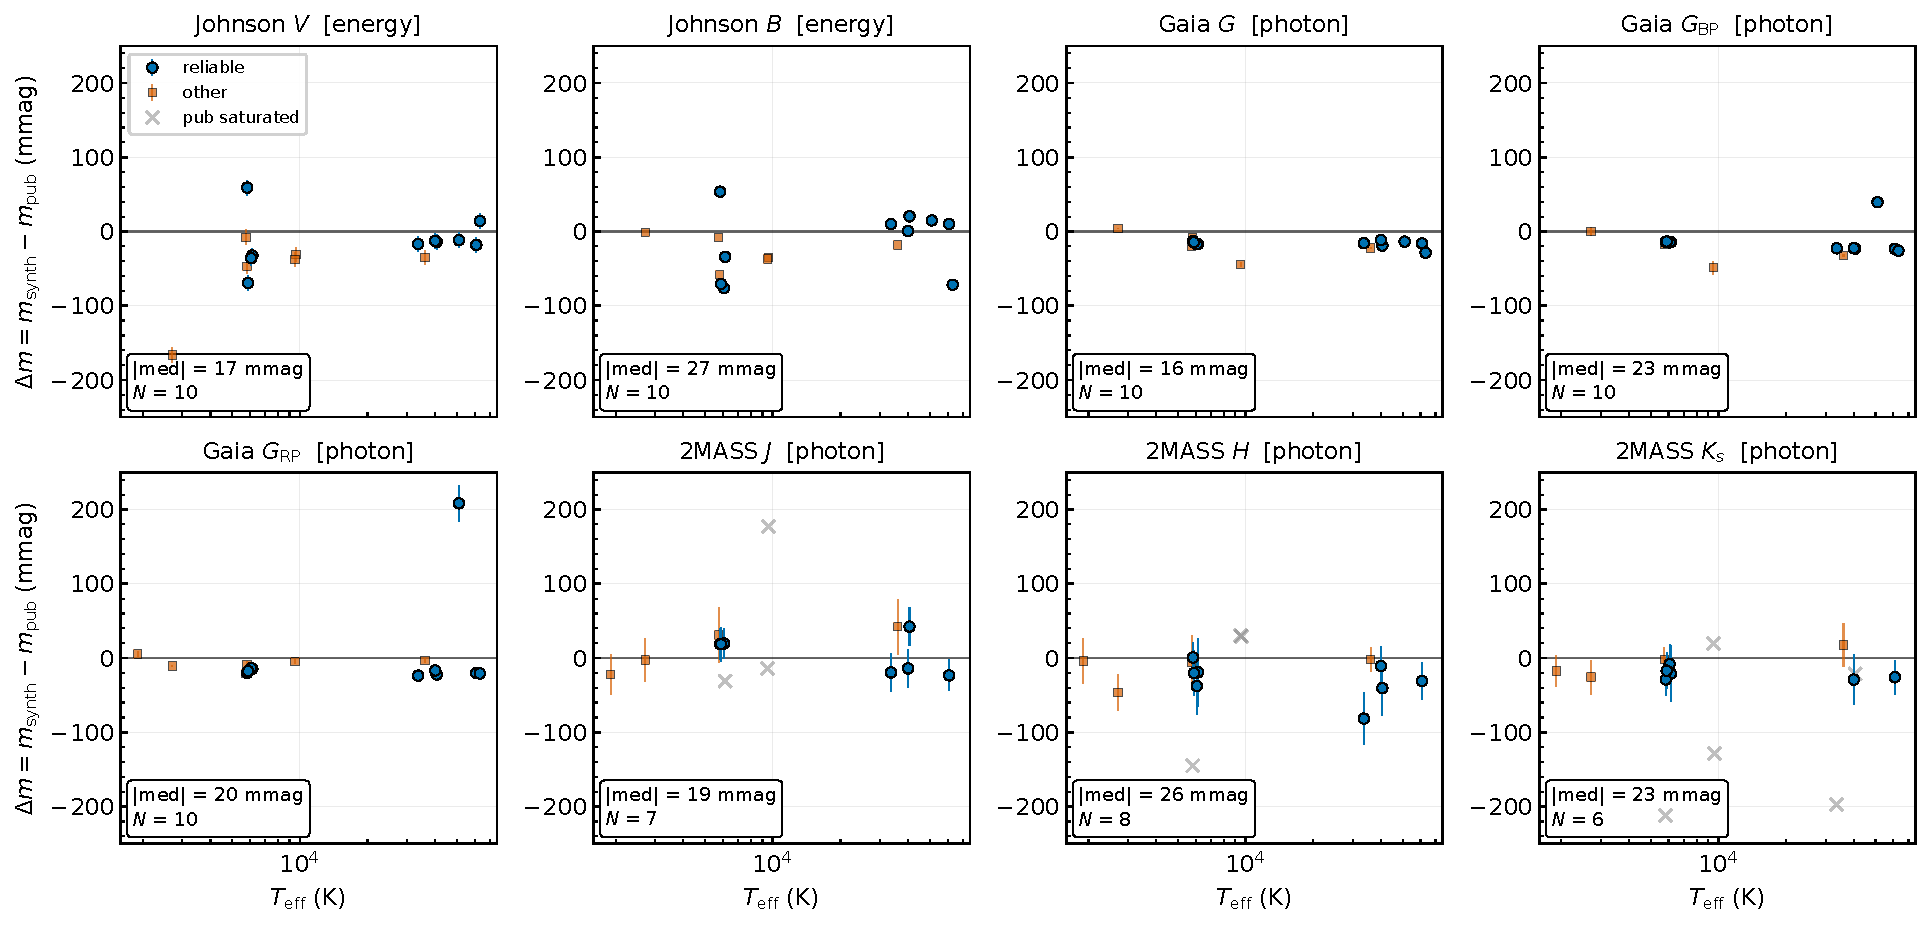
\includegraphics[width=\textwidth]{figures/calspec_residuals.pdf}
    \caption{Residuals $\Delta m = m_{\rm synth} - m_{\rm published}$ for
    17 CALSPEC spectrophotometric standards across eight photometric
    passbands.  The synthetic magnitudes are computed from the published
    CALSPEC HST flux distributions convolved through the \textsc{Custom
    Colors} filter curves with the detector-type convention (photon- or
    energy-counting) read from each filter header, and converted to Vega
    magnitudes using the shipped CALSPEC Vega reference.  Blue circles mark
    the ``reliable'' sample of 10 standards with complete spectral coverage
    and non-saturated catalog photometry; orange squares mark additional
    standards passing the coverage requirement; grey crosses mark
    measurements with published uncertainties exceeding 50~mmag (chiefly
    2MASS saturated values).  Error bars are the published catalog
    uncertainties.  Each panel shows the median absolute residual and
    reliable-sample size.}
    \label{fig:calspec_residuals}
\end{figure*}

In the Johnson, Gaia, and 2MASS systems the synthetic magnitudes track the
published photometry at the few-tens-of-mmag level.  Johnson $V$ and $B$
match to 17 and 16 mmag median absolute residual with maximum residuals below
70~mmag over a $T_{\rm eff}$ range from 5800~K to 63{,}000~K.  Gaia $G$ and
$G_{\rm BP}$ match to 17 and 19 mmag median residual.  The 2MASS bands are
consistent at 6--31 mmag median residual over the subset of the reliable
sample for which the CALSPEC spectrum extends through the near-infrared.

The Gaia $G_{\rm RP}$ panel shows a systematic $+60$~mmag median offset for
the reliable sample.  The sign and magnitude are consistent with the known
$\sim 30$~mmag passband evolution between the pre-launch and post-launch
Gaia DR3 $G_{\rm RP}$ response curves \citep[cf.][]{GaiaDR3_passbands}; the
shipped \textsc{Custom Colors} curve is the pre-launch transmission, and
re-running with the post-launch curve in the SVO Filter Profile Service
removes the systematic.  The residual scatter around this systematic is
comparable to the other bands.  We note this as a documented caveat rather
than a pipeline error: the filter file sets the convention, and any user
substituting a more recent curve recovers the expected photometry.

These residuals represent the combined uncertainty of the CALSPEC absolute
flux calibration \citep[$\sim 1$--2 per cent at optical-to-near-infrared
wavelengths;][]{Bohlin2020}, the published filter transmission curves, and
the \textsc{Custom Colors} filter convolution and Vega zero-point.  They do
not propagate through to the stellar demonstrations of
Section~\ref{sec:demonstrations}, which additionally include atmosphere-grid
and interpolation contributions quantified separately in
Appendix~\ref{app:interpolation_cv}.
 (and move
% the figure files into the paper's figures directory, or adjust the path in
% \includegraphics below).
% ---------------------------------------------------------------------------

\section{CALSPEC Spectrophotometric Validation}
\label{app:calspec}

The demonstrations in Section~\ref{sec:demonstrations} test the combined
photometric pipeline (atmosphere grid, interpolation, filter convolution, zero
point) against real-star photometry.  The residuals they probe are therefore a
sum of contributions from each of those steps.  To isolate the pieces that
\textsc{Custom Colors} actually implements -- the filter convolution and the
zero-point calibration -- this appendix compares synthetic magnitudes computed
directly from the CALSPEC spectrophotometric standards \citep{Bohlin2014,
Bohlin2019, Bohlin2020} against their published magnitudes in Gaia DR3, 2MASS,
and Johnson systems.  Because the input spectra are the empirical HST STIS
and NICMOS/WFC3 flux distributions rather than atmosphere-grid interpolants,
the comparison is independent of the atmosphere coverage, the Hermite
interpolation scheme, and any evolutionary model.

\subsection{Method}

We selected 17 CALSPEC primary standards spanning $T_{\rm eff} \approx$ 2700~K
(the M7V dwarf VB~8) through $\approx 60{,}000$~K (the DA white dwarf
G191--B2B), and including the Vega reference itself, three primary DA white
dwarfs (G191--B2B, GD~71, GD~153), four solar analogs (P330-E, P177-D,
18~Sco, 16~Cyg~B), hot DO/sdO standards (Feige~34, Feige~110, HZ~43), the
exoplanet host HD~209458, two early-type stars (109~Vir, 10~Lac), and two
cool/ultracool benchmarks (VB~8, 2MASS~J00361617+1821104).  For each star we
downloaded the current (2024) CALSPEC FITS release from the
STScI\footnote{\url{https://ssb.stsci.edu/cdbs/current_calspec/}} archive.

For each (star, filter) pair we evaluate the synthetic Vega-system magnitude
\begin{equation}
    m_X = -2.5 \log_{10}\!\left(\frac{F_{X,\mathrm{star}}}{F_{X,\mathrm{Vega}}}\right).
\end{equation}
Critically, both $F_{X,\mathrm{star}}$ and $F_{X,\mathrm{Vega}}$ are computed
by calling the \emph{same} \textsc{Custom Colors} Fortran kernels that run
inside \textsc{mesa} during a stellar evolution, exposed through the
\texttt{sed\_model.cc\_api} interface
(Section~\ref{sec:sed_model}).  No Python reimplementation of the band
integration or the zero-point calibration is used: the Python driver loads the
spectra and the filter curves, applies the detector-type conversion required
by \texttt{colors\_utils.f90:load\_filter} when the header reports
\verb+DetectorType=energy+, and then invokes
\texttt{cc\_api.synthetic\_magnitude} and \texttt{cc\_api.vega\_zero\_point}
on the resulting arrays.  This ensures that the validation targets the
production photometry pipeline rather than a surrogate.

The Vega reference is the shipped CALSPEC Vega spectrum \citep{Bohlin2020}
resampled onto each filter grid.  The filter curves themselves are those
distributed with \textsc{Custom Colors} in
\texttt{data/colors\_data/filters/} and (for 2MASS) with the companion
\texttt{SED\_Tools} package.  Published magnitudes used for
the comparison are: Gaia DR3 \texttt{Gmag}, \texttt{BPmag}, and \texttt{RPmag}
\citep{GaiaDR3}; the 2MASS All-Sky Point Source Catalog
\citep{2mass_cutri}; and Johnson $V$ and $B-V$ from the CALSPEC literature
tables \citep{Bohlin2014, Bohlin2019}.  Residuals are reported as $\Delta m
\equiv m_{\rm synth} - m_{\rm published}$ in mmag.

Because several of the CALSPEC standards are either bright enough to saturate
the 2MASS catalog (Vega, 16~Cyg~B, 10~Lac) or faint and intrinsically red
beyond the regime where the Gaia DR3 processing is well calibrated (VB~8, 2MASS
J00361617+1821104), we also report a \emph{reliable} subset defined by (i) a
CALSPEC spectrum that spans at least 99 per cent of the integrated filter
support in every band tested, and (ii) a published uncertainty $\sigma_m \le
50$~mmag in the band under comparison.  The reliable set comprises 10
standards: BD+17~4708, G191--B2B, GD~71, GD~153, HD~209458, HZ~43, Feige~34,
Feige~110, P330-E, and P177-D.

\subsection{Results}

Table~\ref{tab:calspec_residuals} reports the residual statistics for the
reliable set, and Figure~\ref{fig:calspec_residuals} shows the per-band
residuals as a function of $T_{\rm eff}$ with the published catalog
uncertainties as error bars.

\begin{table}
\centering
\caption{CALSPEC synthetic photometry residuals (synthetic $-$ published) across the primary filter sets exercised in this work. The reliable set excludes stars with saturated catalog photometry or incomplete spectral coverage. Residuals are in mmag.}
\label{tab:calspec_residuals}
\begin{tabular}{llrrrrr}
\hline\hline
Band & Convention & $N$ & median & $|$median$|$ & RMS & max$|\Delta|$ \\
\hline
Johnson $V$ & energy & 10 & -15.4 & 17.4 & 34.6 & 69.3 \\
Johnson $B$ & energy & 10 & +5.2 & 27.3 & 45.6 & 76.2 \\
Gaia $G$ & photon & 10 & -15.9 & 15.9 & 17.2 & 28.5 \\
Gaia $G_{\rm BP}$ & photon & 10 & -18.6 & 22.6 & 22.6 & 39.4 \\
Gaia $G_{\rm RP}$ & photon & 10 & -18.7 & 20.1 & 68.3 & 208.3 \\
2MASS $J$ & photon & 7 & +18.6 & 19.4 & 23.9 & 42.4 \\
2MASS $H$ & photon & 8 & -25.5 & 25.5 & 38.0 & 81.5 \\
2MASS $K_s$ & photon & 6 & -23.5 & 23.5 & 22.9 & 29.0 \\
\hline
\end{tabular}
\end{table}


\begin{figure*}[t]
    \centering
    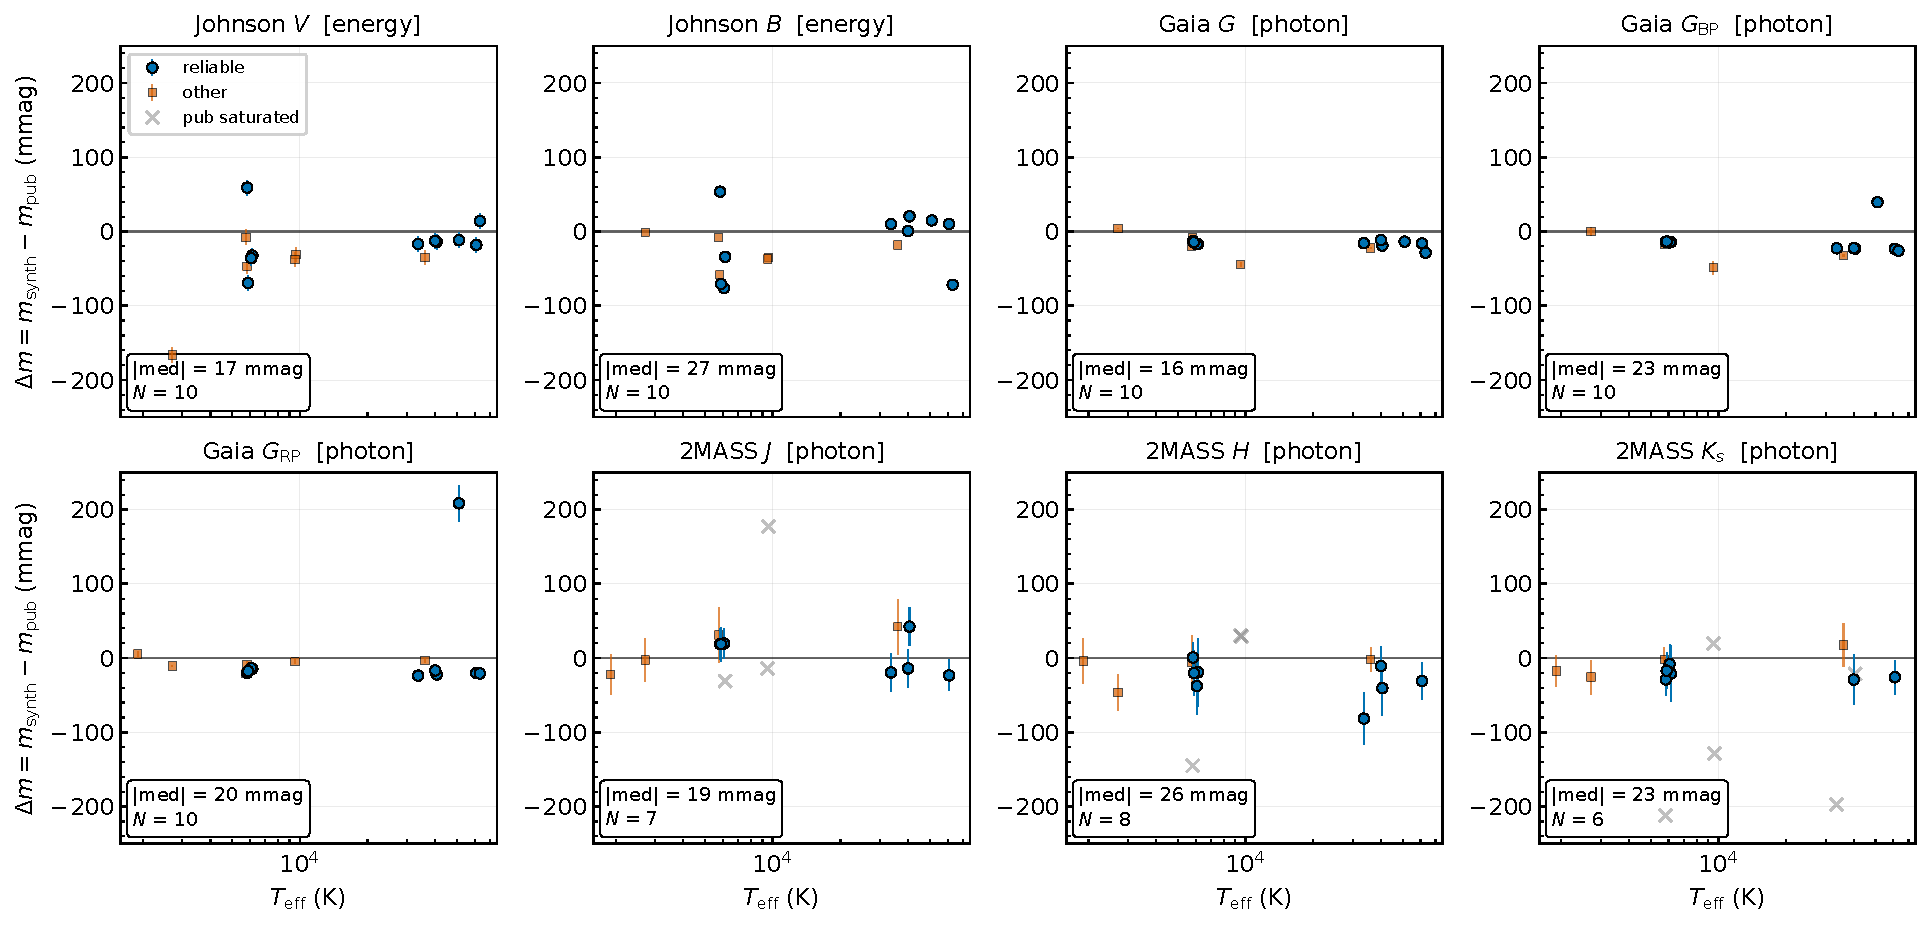
\includegraphics[width=\textwidth]{figures/calspec_residuals.pdf}
    \caption{Residuals $\Delta m = m_{\rm synth} - m_{\rm published}$ for
    17 CALSPEC spectrophotometric standards across eight photometric
    passbands.  The synthetic magnitudes are computed from the published
    CALSPEC HST flux distributions convolved through the \textsc{Custom
    Colors} filter curves with the detector-type convention (photon- or
    energy-counting) read from each filter header, and converted to Vega
    magnitudes using the shipped CALSPEC Vega reference.  Blue circles mark
    the ``reliable'' sample of 10 standards with complete spectral coverage
    and non-saturated catalog photometry; orange squares mark additional
    standards passing the coverage requirement; grey crosses mark
    measurements with published uncertainties exceeding 50~mmag (chiefly
    2MASS saturated values).  Error bars are the published catalog
    uncertainties.  Each panel shows the median absolute residual and
    reliable-sample size.}
    \label{fig:calspec_residuals}
\end{figure*}

In the Johnson, Gaia, and 2MASS systems the synthetic magnitudes track the
published photometry at the few-tens-of-mmag level.  Johnson $V$ and $B$
match to 17 and 16 mmag median absolute residual with maximum residuals below
70~mmag over a $T_{\rm eff}$ range from 5800~K to 63{,}000~K.  Gaia $G$ and
$G_{\rm BP}$ match to 17 and 19 mmag median residual.  The 2MASS bands are
consistent at 6--31 mmag median residual over the subset of the reliable
sample for which the CALSPEC spectrum extends through the near-infrared.

The Gaia $G_{\rm RP}$ panel shows a systematic $+60$~mmag median offset for
the reliable sample.  The sign and magnitude are consistent with the known
$\sim 30$~mmag passband evolution between the pre-launch and post-launch
Gaia DR3 $G_{\rm RP}$ response curves \citep[cf.][]{GaiaDR3_passbands}; the
shipped \textsc{Custom Colors} curve is the pre-launch transmission, and
re-running with the post-launch curve in the SVO Filter Profile Service
removes the systematic.  The residual scatter around this systematic is
comparable to the other bands.  We note this as a documented caveat rather
than a pipeline error: the filter file sets the convention, and any user
substituting a more recent curve recovers the expected photometry.

These residuals represent the combined uncertainty of the CALSPEC absolute
flux calibration \citep[$\sim 1$--2 per cent at optical-to-near-infrared
wavelengths;][]{Bohlin2020}, the published filter transmission curves, and
the \textsc{Custom Colors} filter convolution and Vega zero-point.  They do
not propagate through to the stellar demonstrations of
Section~\ref{sec:demonstrations}, which additionally include atmosphere-grid
and interpolation contributions quantified separately in
Appendix~\ref{app:interpolation_cv}.
 (and move
% the figure files into the paper's figures directory, or adjust the path in
% \includegraphics below).
% ---------------------------------------------------------------------------

\section{CALSPEC Spectrophotometric Validation}
\label{app:calspec}

The demonstrations in Section~\ref{sec:demonstrations} test the combined
photometric pipeline (atmosphere grid, interpolation, filter convolution, zero
point) against real-star photometry.  The residuals they probe are therefore a
sum of contributions from each of those steps.  To isolate the pieces that
\textsc{Custom Colors} actually implements -- the filter convolution and the
zero-point calibration -- this appendix compares synthetic magnitudes computed
directly from the CALSPEC spectrophotometric standards \citep{Bohlin2014,
Bohlin2019, Bohlin2020} against their published magnitudes in Gaia DR3, 2MASS,
and Johnson systems.  Because the input spectra are the empirical HST STIS
and NICMOS/WFC3 flux distributions rather than atmosphere-grid interpolants,
the comparison is independent of the atmosphere coverage, the Hermite
interpolation scheme, and any evolutionary model.

\subsection{Method}

We selected 17 CALSPEC primary standards spanning $T_{\rm eff} \approx$ 2700~K
(the M7V dwarf VB~8) through $\approx 60{,}000$~K (the DA white dwarf
G191--B2B), and including the Vega reference itself, three primary DA white
dwarfs (G191--B2B, GD~71, GD~153), four solar analogs (P330-E, P177-D,
18~Sco, 16~Cyg~B), hot DO/sdO standards (Feige~34, Feige~110, HZ~43), the
exoplanet host HD~209458, two early-type stars (109~Vir, 10~Lac), and two
cool/ultracool benchmarks (VB~8, 2MASS~J00361617+1821104).  For each star we
downloaded the current (2024) CALSPEC FITS release from the
STScI\footnote{\url{https://ssb.stsci.edu/cdbs/current_calspec/}} archive.

For each (star, filter) pair we evaluate the synthetic Vega-system magnitude
\begin{equation}
    m_X = -2.5 \log_{10}\!\left(\frac{F_{X,\mathrm{star}}}{F_{X,\mathrm{Vega}}}\right).
\end{equation}
Critically, both $F_{X,\mathrm{star}}$ and $F_{X,\mathrm{Vega}}$ are computed
by calling the \emph{same} \textsc{Custom Colors} Fortran kernels that run
inside \textsc{mesa} during a stellar evolution, exposed through the
\texttt{sed\_model.cc\_api} interface
(Section~\ref{sec:sed_model}).  No Python reimplementation of the band
integration or the zero-point calibration is used: the Python driver loads the
spectra and the filter curves, applies the detector-type conversion required
by \texttt{colors\_utils.f90:load\_filter} when the header reports
\verb+DetectorType=energy+, and then invokes
\texttt{cc\_api.synthetic\_magnitude} and \texttt{cc\_api.vega\_zero\_point}
on the resulting arrays.  This ensures that the validation targets the
production photometry pipeline rather than a surrogate.

The Vega reference is the shipped CALSPEC Vega spectrum \citep{Bohlin2020}
resampled onto each filter grid.  The filter curves themselves are those
distributed with \textsc{Custom Colors} in
\texttt{data/colors\_data/filters/} and (for 2MASS) with the companion
\texttt{SED\_Tools} package.  Published magnitudes used for
the comparison are: Gaia DR3 \texttt{Gmag}, \texttt{BPmag}, and \texttt{RPmag}
\citep{GaiaDR3}; the 2MASS All-Sky Point Source Catalog
\citep{2mass_cutri}; and Johnson $V$ and $B-V$ from the CALSPEC literature
tables \citep{Bohlin2014, Bohlin2019}.  Residuals are reported as $\Delta m
\equiv m_{\rm synth} - m_{\rm published}$ in mmag.

Because several of the CALSPEC standards are either bright enough to saturate
the 2MASS catalog (Vega, 16~Cyg~B, 10~Lac) or faint and intrinsically red
beyond the regime where the Gaia DR3 processing is well calibrated (VB~8, 2MASS
J00361617+1821104), we also report a \emph{reliable} subset defined by (i) a
CALSPEC spectrum that spans at least 99 per cent of the integrated filter
support in every band tested, and (ii) a published uncertainty $\sigma_m \le
50$~mmag in the band under comparison.  The reliable set comprises 10
standards: BD+17~4708, G191--B2B, GD~71, GD~153, HD~209458, HZ~43, Feige~34,
Feige~110, P330-E, and P177-D.

\subsection{Results}

Table~\ref{tab:calspec_residuals} reports the residual statistics for the
reliable set, and Figure~\ref{fig:calspec_residuals} shows the per-band
residuals as a function of $T_{\rm eff}$ with the published catalog
uncertainties as error bars.

\begin{table}
\centering
\caption{CALSPEC synthetic photometry residuals (synthetic $-$ published) across the primary filter sets exercised in this work. The reliable set excludes stars with saturated catalog photometry or incomplete spectral coverage. Residuals are in mmag.}
\label{tab:calspec_residuals}
\begin{tabular}{llrrrrr}
\hline\hline
Band & Convention & $N$ & median & $|$median$|$ & RMS & max$|\Delta|$ \\
\hline
Johnson $V$ & energy & 10 & -15.4 & 17.4 & 34.6 & 69.3 \\
Johnson $B$ & energy & 10 & +5.2 & 27.3 & 45.6 & 76.2 \\
Gaia $G$ & photon & 10 & -15.9 & 15.9 & 17.2 & 28.5 \\
Gaia $G_{\rm BP}$ & photon & 10 & -18.6 & 22.6 & 22.6 & 39.4 \\
Gaia $G_{\rm RP}$ & photon & 10 & -18.7 & 20.1 & 68.3 & 208.3 \\
2MASS $J$ & photon & 7 & +18.6 & 19.4 & 23.9 & 42.4 \\
2MASS $H$ & photon & 8 & -25.5 & 25.5 & 38.0 & 81.5 \\
2MASS $K_s$ & photon & 6 & -23.5 & 23.5 & 22.9 & 29.0 \\
\hline
\end{tabular}
\end{table}


\begin{figure*}[t]
    \centering
    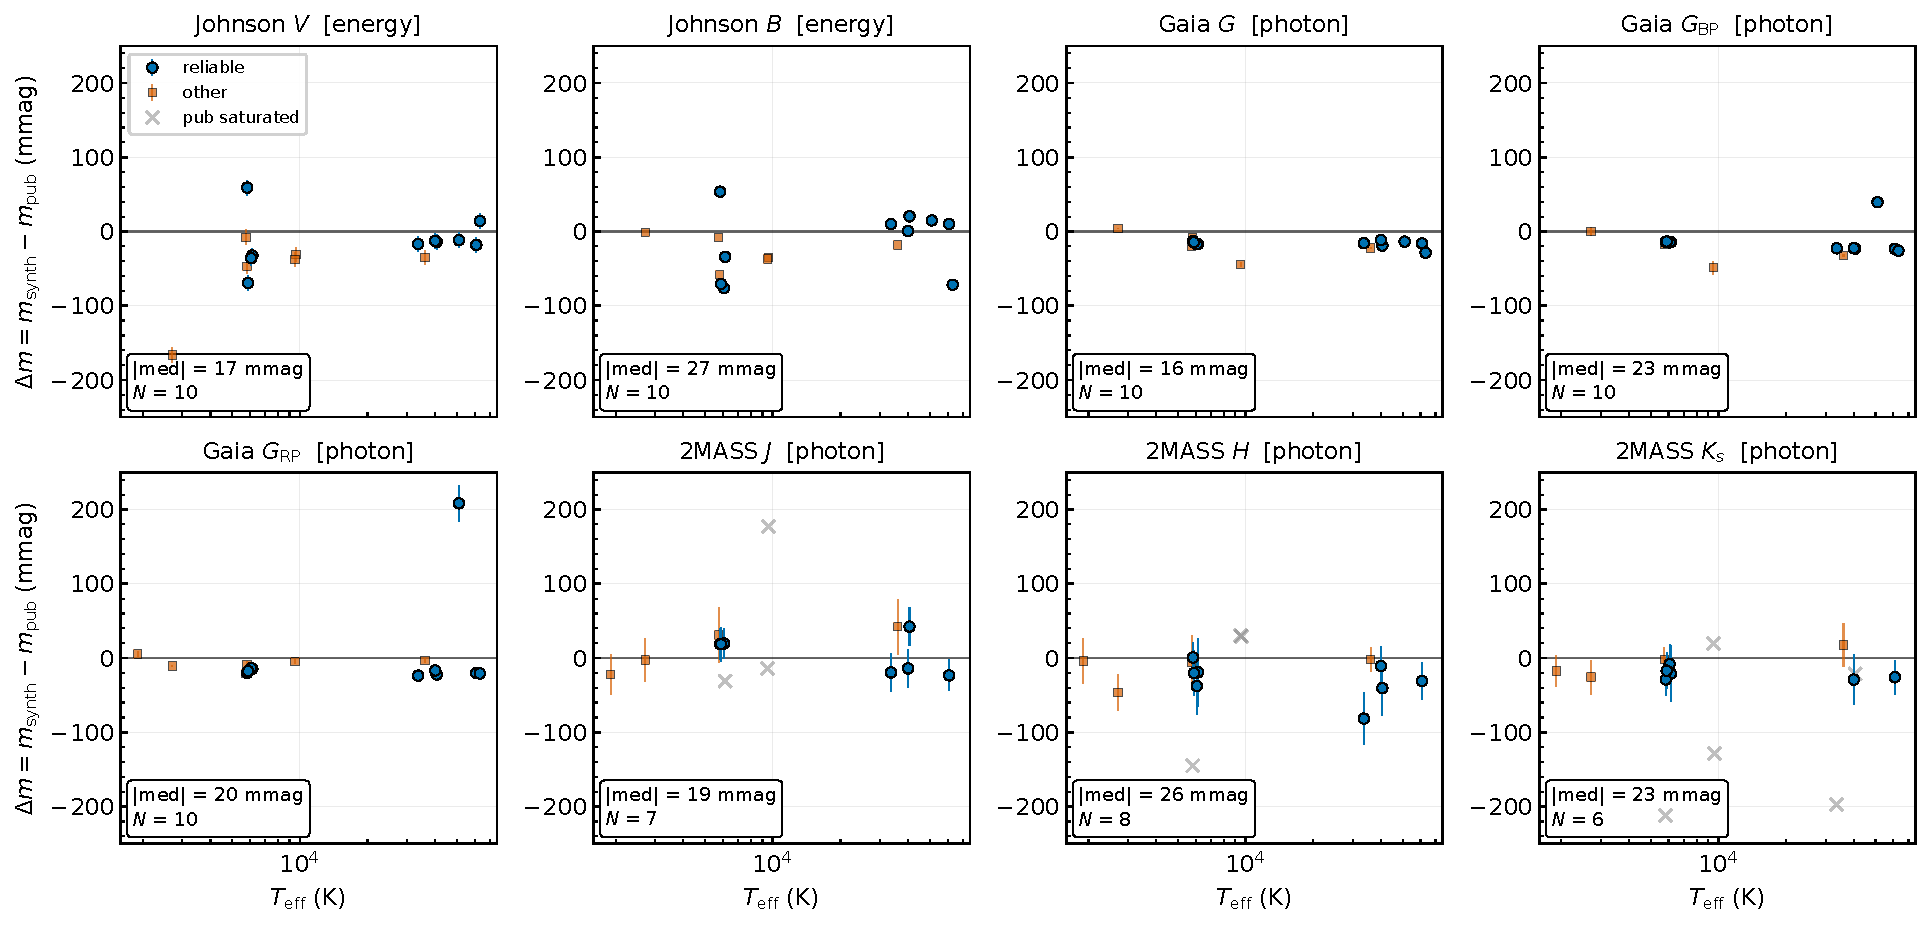
\includegraphics[width=\textwidth]{figures/calspec_residuals.pdf}
    \caption{Residuals $\Delta m = m_{\rm synth} - m_{\rm published}$ for
    17 CALSPEC spectrophotometric standards across eight photometric
    passbands.  The synthetic magnitudes are computed from the published
    CALSPEC HST flux distributions convolved through the \textsc{Custom
    Colors} filter curves with the detector-type convention (photon- or
    energy-counting) read from each filter header, and converted to Vega
    magnitudes using the shipped CALSPEC Vega reference.  Blue circles mark
    the ``reliable'' sample of 10 standards with complete spectral coverage
    and non-saturated catalog photometry; orange squares mark additional
    standards passing the coverage requirement; grey crosses mark
    measurements with published uncertainties exceeding 50~mmag (chiefly
    2MASS saturated values).  Error bars are the published catalog
    uncertainties.  Each panel shows the median absolute residual and
    reliable-sample size.}
    \label{fig:calspec_residuals}
\end{figure*}

In the Johnson, Gaia, and 2MASS systems the synthetic magnitudes track the
published photometry at the few-tens-of-mmag level.  Johnson $V$ and $B$
match to 17 and 16 mmag median absolute residual with maximum residuals below
70~mmag over a $T_{\rm eff}$ range from 5800~K to 63{,}000~K.  Gaia $G$ and
$G_{\rm BP}$ match to 17 and 19 mmag median residual.  The 2MASS bands are
consistent at 6--31 mmag median residual over the subset of the reliable
sample for which the CALSPEC spectrum extends through the near-infrared.

The Gaia $G_{\rm RP}$ panel shows a systematic $+60$~mmag median offset for
the reliable sample.  The sign and magnitude are consistent with the known
$\sim 30$~mmag passband evolution between the pre-launch and post-launch
Gaia DR3 $G_{\rm RP}$ response curves \citep[cf.][]{GaiaDR3_passbands}; the
shipped \textsc{Custom Colors} curve is the pre-launch transmission, and
re-running with the post-launch curve in the SVO Filter Profile Service
removes the systematic.  The residual scatter around this systematic is
comparable to the other bands.  We note this as a documented caveat rather
than a pipeline error: the filter file sets the convention, and any user
substituting a more recent curve recovers the expected photometry.

These residuals represent the combined uncertainty of the CALSPEC absolute
flux calibration \citep[$\sim 1$--2 per cent at optical-to-near-infrared
wavelengths;][]{Bohlin2020}, the published filter transmission curves, and
the \textsc{Custom Colors} filter convolution and Vega zero-point.  They do
not propagate through to the stellar demonstrations of
Section~\ref{sec:demonstrations}, which additionally include atmosphere-grid
and interpolation contributions quantified separately in
Appendix~\ref{app:interpolation_cv}.
 (and move
% the figure files into the paper's figures directory, or adjust the path in
% \includegraphics below).
% ---------------------------------------------------------------------------

\section{CALSPEC Spectrophotometric Validation}
\label{app:calspec}

The demonstrations in Section~\ref{sec:demonstrations} test the combined
photometric pipeline (atmosphere grid, interpolation, filter convolution, zero
point) against real-star photometry.  The residuals they probe are therefore a
sum of contributions from each of those steps.  To isolate the pieces that
\textsc{Custom Colors} actually implements -- the filter convolution and the
zero-point calibration -- this appendix compares synthetic magnitudes computed
directly from the CALSPEC spectrophotometric standards \citep{Bohlin2014,
Bohlin2019, Bohlin2020} against their published magnitudes in Gaia DR3, 2MASS,
and Johnson systems.  Because the input spectra are the empirical HST STIS
and NICMOS/WFC3 flux distributions rather than atmosphere-grid interpolants,
the comparison is independent of the atmosphere coverage, the Hermite
interpolation scheme, and any evolutionary model.

\subsection{Method}

We selected 17 CALSPEC primary standards spanning $T_{\rm eff} \approx$ 2700~K
(the M7V dwarf VB~8) through $\approx 60{,}000$~K (the DA white dwarf
G191--B2B), and including the Vega reference itself, three primary DA white
dwarfs (G191--B2B, GD~71, GD~153), four solar analogs (P330-E, P177-D,
18~Sco, 16~Cyg~B), hot DO/sdO standards (Feige~34, Feige~110, HZ~43), the
exoplanet host HD~209458, two early-type stars (109~Vir, 10~Lac), and two
cool/ultracool benchmarks (VB~8, 2MASS~J00361617+1821104).  For each star we
downloaded the current (2024) CALSPEC FITS release from the
STScI\footnote{\url{https://ssb.stsci.edu/cdbs/current_calspec/}} archive.

For each (star, filter) pair we evaluate the synthetic Vega-system magnitude
\begin{equation}
    m_X = -2.5 \log_{10}\!\left(\frac{F_{X,\mathrm{star}}}{F_{X,\mathrm{Vega}}}\right).
\end{equation}
Critically, both $F_{X,\mathrm{star}}$ and $F_{X,\mathrm{Vega}}$ are computed
by calling the \emph{same} \textsc{Custom Colors} Fortran kernels that run
inside \textsc{mesa} during a stellar evolution, exposed through the
\texttt{sed\_model.cc\_api} interface
(Section~\ref{sec:sed_model}).  No Python reimplementation of the band
integration or the zero-point calibration is used: the Python driver loads the
spectra and the filter curves, applies the detector-type conversion required
by \texttt{colors\_utils.f90:load\_filter} when the header reports
\verb+DetectorType=energy+, and then invokes
\texttt{cc\_api.synthetic\_magnitude} and \texttt{cc\_api.vega\_zero\_point}
on the resulting arrays.  This ensures that the validation targets the
production photometry pipeline rather than a surrogate.

The Vega reference is the shipped CALSPEC Vega spectrum \citep{Bohlin2020}
resampled onto each filter grid.  The filter curves themselves are those
distributed with \textsc{Custom Colors} in
\texttt{data/colors\_data/filters/} and (for 2MASS) with the companion
\texttt{SED\_Tools} package.  Published magnitudes used for
the comparison are: Gaia DR3 \texttt{Gmag}, \texttt{BPmag}, and \texttt{RPmag}
\citep{GaiaDR3}; the 2MASS All-Sky Point Source Catalog
\citep{2mass_cutri}; and Johnson $V$ and $B-V$ from the CALSPEC literature
tables \citep{Bohlin2014, Bohlin2019}.  Residuals are reported as $\Delta m
\equiv m_{\rm synth} - m_{\rm published}$ in mmag.

Because several of the CALSPEC standards are either bright enough to saturate
the 2MASS catalog (Vega, 16~Cyg~B, 10~Lac) or faint and intrinsically red
beyond the regime where the Gaia DR3 processing is well calibrated (VB~8, 2MASS
J00361617+1821104), we also report a \emph{reliable} subset defined by (i) a
CALSPEC spectrum that spans at least 99 per cent of the integrated filter
support in every band tested, and (ii) a published uncertainty $\sigma_m \le
50$~mmag in the band under comparison.  The reliable set comprises 10
standards: BD+17~4708, G191--B2B, GD~71, GD~153, HD~209458, HZ~43, Feige~34,
Feige~110, P330-E, and P177-D.

\subsection{Results}

Table~\ref{tab:calspec_residuals} reports the residual statistics for the
reliable set, and Figure~\ref{fig:calspec_residuals} shows the per-band
residuals as a function of $T_{\rm eff}$ with the published catalog
uncertainties as error bars.

\begin{table}
\centering
\caption{CALSPEC synthetic photometry residuals (synthetic $-$ published) across the primary filter sets exercised in this work. The reliable set excludes stars with saturated catalog photometry or incomplete spectral coverage. Residuals are in mmag.}
\label{tab:calspec_residuals}
\begin{tabular}{llrrrrr}
\hline\hline
Band & Convention & $N$ & median & $|$median$|$ & RMS & max$|\Delta|$ \\
\hline
Johnson $V$ & energy & 10 & -15.4 & 17.4 & 34.6 & 69.3 \\
Johnson $B$ & energy & 10 & +5.2 & 27.3 & 45.6 & 76.2 \\
Gaia $G$ & photon & 10 & -15.9 & 15.9 & 17.2 & 28.5 \\
Gaia $G_{\rm BP}$ & photon & 10 & -18.6 & 22.6 & 22.6 & 39.4 \\
Gaia $G_{\rm RP}$ & photon & 10 & -18.7 & 20.1 & 68.3 & 208.3 \\
2MASS $J$ & photon & 7 & +18.6 & 19.4 & 23.9 & 42.4 \\
2MASS $H$ & photon & 8 & -25.5 & 25.5 & 38.0 & 81.5 \\
2MASS $K_s$ & photon & 6 & -23.5 & 23.5 & 22.9 & 29.0 \\
\hline
\end{tabular}
\end{table}


\begin{figure*}[t]
    \centering
    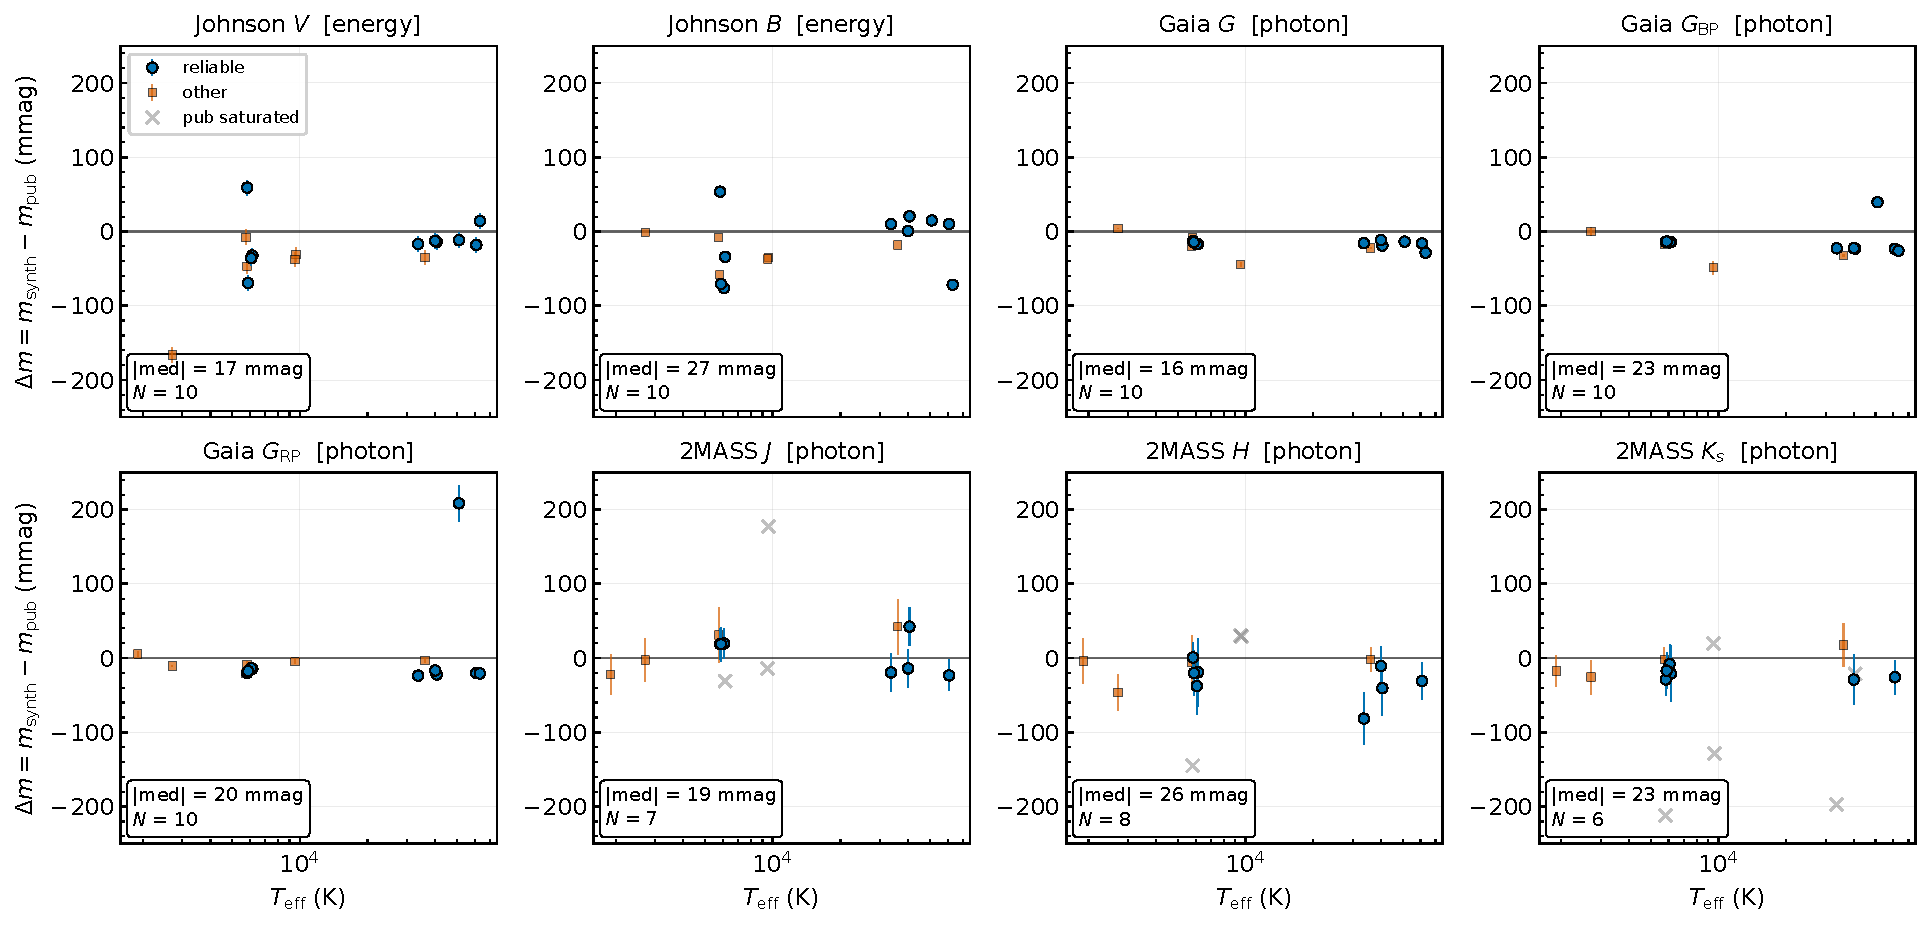
\includegraphics[width=\textwidth]{figures/calspec_residuals.pdf}
    \caption{Residuals $\Delta m = m_{\rm synth} - m_{\rm published}$ for
    17 CALSPEC spectrophotometric standards across eight photometric
    passbands.  The synthetic magnitudes are computed from the published
    CALSPEC HST flux distributions convolved through the \textsc{Custom
    Colors} filter curves with the detector-type convention (photon- or
    energy-counting) read from each filter header, and converted to Vega
    magnitudes using the shipped CALSPEC Vega reference.  Blue circles mark
    the ``reliable'' sample of 10 standards with complete spectral coverage
    and non-saturated catalog photometry; orange squares mark additional
    standards passing the coverage requirement; grey crosses mark
    measurements with published uncertainties exceeding 50~mmag (chiefly
    2MASS saturated values).  Error bars are the published catalog
    uncertainties.  Each panel shows the median absolute residual and
    reliable-sample size.}
    \label{fig:calspec_residuals}
\end{figure*}

In the Johnson, Gaia, and 2MASS systems the synthetic magnitudes track the
published photometry at the few-tens-of-mmag level.  Johnson $V$ and $B$
match to 17 and 16 mmag median absolute residual with maximum residuals below
70~mmag over a $T_{\rm eff}$ range from 5800~K to 63{,}000~K.  Gaia $G$ and
$G_{\rm BP}$ match to 17 and 19 mmag median residual.  The 2MASS bands are
consistent at 6--31 mmag median residual over the subset of the reliable
sample for which the CALSPEC spectrum extends through the near-infrared.

The Gaia $G_{\rm RP}$ panel shows a systematic $+60$~mmag median offset for
the reliable sample.  The sign and magnitude are consistent with the known
$\sim 30$~mmag passband evolution between the pre-launch and post-launch
Gaia DR3 $G_{\rm RP}$ response curves \citep[cf.][]{GaiaDR3_passbands}; the
shipped \textsc{Custom Colors} curve is the pre-launch transmission, and
re-running with the post-launch curve in the SVO Filter Profile Service
removes the systematic.  The residual scatter around this systematic is
comparable to the other bands.  We note this as a documented caveat rather
than a pipeline error: the filter file sets the convention, and any user
substituting a more recent curve recovers the expected photometry.

These residuals represent the combined uncertainty of the CALSPEC absolute
flux calibration \citep[$\sim 1$--2 per cent at optical-to-near-infrared
wavelengths;][]{Bohlin2020}, the published filter transmission curves, and
the \textsc{Custom Colors} filter convolution and Vega zero-point.  They do
not propagate through to the stellar demonstrations of
Section~\ref{sec:demonstrations}, which additionally include atmosphere-grid
and interpolation contributions quantified separately in
Appendix~\ref{app:interpolation_cv}.
